\subsection{Predictive quality at matched width}
Table~\ref{tab:primary} reports the eight benchmark sources without pooling AUC and $R^2$. On Spambase, the row-split comparison favoured voting over $F$ by a median 0.039 AUC with either learner, at greater cost. In each split, 118--133 of the 1,151 test rows had feature vectors also present in training. We repeated training with identical 57-coordinate vectors assigned to the same fold and weighted each distinct test vector equally. The paired AUC difference was then negative for ridge on all five folds (median $-0.011$, range $-0.036$ to $-0.005$) and positive for trees on all five (median $+0.021$, range $+0.009$ to $+0.048$). Simply removing the overlapping rows from the original test folds left both comparisons positive; fitting again on group-disjoint folds changed the sign for ridge. Relative to using all columns, grouped AUC fell by a median 0.086 with ridge and 0.045 with trees. For the Gisette ridge model, voting reduced the median paired total time to 0.63 of that for $F$ selection, with a paired AUC change of $-0.002$. The same conclusion did not hold across sources. On Madelon with a tree learner, the median paired AUC change against $F$ was $-0.191$. On Diabetes a one-column budget is particularly restrictive: the median ridge $R^2$ was 0.021 for voting and 0.298 for $F$. On Communities and Crime those medians were 0.291 and 0.475, respectively. Discretizing the response for the neighbour search can discard distance information relevant to a continuous loss. This experiment does not isolate binning from the other differences between selectors.

\begin{table}[tbp]
\centering\small
\caption{Median held-out performance on five splits. Entries are macro or binary ROC AUC for the six classification sources, and $R^2$ for the last two sources. Full uses all columns. ET denotes impurity ranking by extremely randomized trees; P+ET screens to 40\% before ET selects the same final width.}
\label{tab:primary}
\setlength{\tabcolsep}{3pt}
\begin{tabular}{@{}llrrrrrr@{}}
\toprule
Dataset & Fit & Full & Uniform & $F$ & ET & Pivotal & P+ET\\
\midrule
Breast cancer & Ridge & 0.999 & 0.986 & 0.995 & 0.993 & 0.987 & 0.993 \\
 & Trees & 0.999 & 0.982 & 0.991 & 0.988 & 0.982 & 0.985 \\
Digits & Ridge & 0.991 & 0.870 & 0.936 & 0.937 & 0.933 & 0.943 \\
 & Trees & 1.000 & 0.891 & 0.973 & 0.977 & 0.974 & 0.984 \\
Madelon & Ridge & 0.572 & 0.540 & 0.596 & 0.609 & 0.609 & 0.619 \\
 & Trees & 0.706 & 0.529 & 0.851 & 0.931 & 0.660 & 0.791 \\
Spambase & Ridge & 0.951 & 0.799 & 0.884 & 0.911 & 0.914 & 0.908 \\
 & Trees & 0.989 & 0.807 & 0.906 & 0.919 & 0.948 & 0.955 \\
ISOLET & Ridge & 0.994 & 0.978 & 0.969 & 0.982 & 0.982 & 0.981 \\
 & Trees & 0.998 & 0.993 & 0.991 & 0.995 & 0.993 & 0.995 \\
Gisette & Ridge & 0.967 & 0.980 & 0.995 & 0.996 & 0.993 & 0.996 \\
 & Trees & 0.997 & 0.991 & 0.997 & 0.997 & 0.996 & 0.997 \\
Diabetes & Ridge & 0.475 & 0.162 & 0.298 & 0.298 & 0.021 & 0.185 \\
 & Trees & 0.481 & -0.009 & -0.009 & -0.009 & -0.057 & -0.015 \\
Communities and Crime & Ridge & 0.543 & 0.421 & 0.475 & 0.475 & 0.291 & 0.480 \\
 & Trees & 0.547 & 0.453 & 0.455 & 0.459 & 0.407 & 0.490
\\
\bottomrule
\end{tabular}
\end{table}

\subsection{When does a first screen pay for itself?}
Screening before a forest changes the cost of ranking features on the full table. On ISOLET the extra screen and final ridge fit together took a median of 0.64 times as long as the corresponding pipeline using direct impurity ranking; for a final tree fit the ratio was 0.72. On Gisette the corresponding ratios were 0.39 and 0.45. All five splits met the timing and quality criteria against the direct tree selector in each of these four comparisons. When the same split also had to meet the quality tolerances against the full-width learner, Gisette still passed on all five splits with each learner and ISOLET passed on none. The comparator in each case fits the same impurity selector directly on the full input and passes the same number of columns downstream. End-to-end ratios account for both the screen and the downstream fit. The relative reduction shrinks when downstream fitting consumes more of the total time.

The forest on Madelon provides a counterexample. Screening its input improved the median time ratio to 0.84 with a final tree learner, but median paired AUC fell by 0.139. Across splits its smallest loss was 0.021, already outside the stated AUC tolerance (Table~\ref{tab:prefilter}). When a first-stage filter removes a coordinate, the forest cannot use it to construct a split or interaction. A faster front end therefore has to be evaluated with the selector it precedes.

\begin{table}[tbp]
\centering\small
\caption{Screening before ET versus direct ET. $\Delta$ is the median paired difference in held-out AUC or $R^2$; the last two columns give its range over five splits. Time is the median paired end-to-end ratio. ET counts splits meeting the timing and quality criteria against direct ET. Both also requires acceptable quality against the full-width learner.}
\label{tab:prefilter}
\setlength{\tabcolsep}{3pt}
\begin{tabular}{@{}llrrrrrr@{}}
\toprule Dataset & Fit & $\Delta$ & Time & ET / 5 & Both / 5 & Min $\Delta$ & Max $\Delta$\\
\midrule
Breast cancer & Ridge & +0.002 & 1.05 & 0 & 0 & -0.001 & +0.004 \\
 & Trees & +0.001 & 1.03 & 0 & 0 & -0.006 & +0.006 \\
Digits & Ridge & +0.006 & 1.00 & 1 & 0 & -0.006 & +0.018 \\
 & Trees & +0.006 & 0.98 & 0 & 0 & -0.001 & +0.012 \\
Madelon & Ridge & +0.007 & 0.74 & 4 & 4 & -0.007 & +0.017 \\
 & Trees & -0.139 & 0.84 & 0 & 0 & -0.201 & -0.021 \\
Spambase & Ridge & 0.000 & 0.77 & 1 & 0 & -0.021 & +0.045 \\
 & Trees & +0.026 & 0.86 & 1 & 0 & +0.008 & +0.036 \\
ISOLET & Ridge & 0.000 & 0.64 & 5 & 0 & -0.003 & +0.001 \\
 & Trees & 0.000 & 0.72 & 5 & 0 & 0.000 & +0.001 \\
Gisette & Ridge & 0.000 & 0.39 & 5 & 5 & 0.000 & +0.001 \\
 & Trees & 0.000 & 0.45 & 5 & 5 & 0.000 & +0.001 \\
Diabetes & Ridge & -0.176 & 0.93 & 0 & 0 & -0.196 & 0.000 \\
 & Trees & 0.000 & 0.95 & 0 & 0 & -0.268 & +0.117 \\
Communities and Crime & Ridge & -0.009 & 0.75 & 3 & 0 & -0.068 & +0.005 \\
 & Trees & -0.005 & 0.83 & 2 & 0 & -0.021 & +0.036
\\
\bottomrule
\end{tabular}
\end{table}

\begin{figure}[tbp]
\centering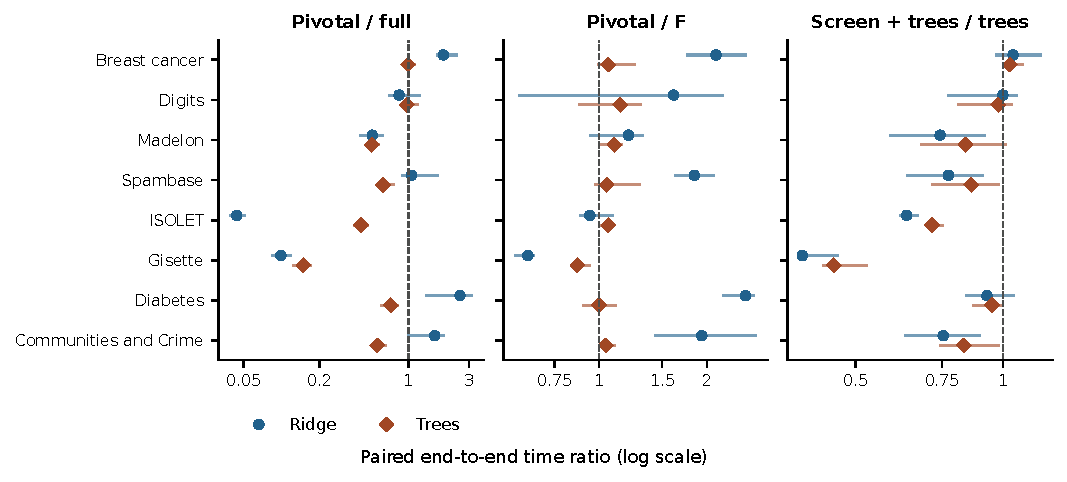
\includegraphics[width=\linewidth]{time-ratios}
\caption{Paired run-time ratios on identical train and test rows. Points show medians and lines show ranges over five splits. Values below one favour the numerator. The first two panels evaluate pivotal minPI used directly; the third measures the additional screen before the same tree selector.}
\label{fig:time}
\end{figure}
Figure~\ref{fig:time} separates two questions about speed. Reducing the number of columns may shorten the final model fit relative to using all columns. At matched width, a reduction in fit time has to compensate for any additional cost of computing the ranking. For example, on Spambase a ridge model with the voting screen took 1.84 times the paired time of a ridge model using $F$ selection. Subsecond results are sensitive to the numerical libraries and machine load.

\subsection{Which coalition sizes affect selection?}
The minimum returned exactly the same top-budget set as the largest designated layer on all 30 benchmark classification splits and all 15 simulated classification splits. It agreed on five of ten regression splits, giving 50 agreements among 55 comparisons in total. This equality concerns the selected sets. Individual features can attain their minimum at other sizes even when the selected set stays the same. The likelihood of a pivotal tie often falls as more peers cast ballots, which gives the largest layer a smaller positive gain on many features. The finite-population argument in Theorem~\ref{thm:agreement} explains such a tendency for nonabstaining rows and even sizes; it does not force agreement for a general vote matrix. The matched comparison provides no independent classification gain from taking a minimum over the three chosen sizes.

\begin{table}[tbp]
\centering\small
\caption{Median within-split Jaccard similarity of selected features to pivotal minPI, on each benchmark source. Mean averages across layers, Vote uses only signed ballots, Last uses the largest available layer, MC samples 32 peer sets per nonempty layer, and Raw averages the original signed distance differences before ternary coding. Error is the median of the per-split maximum absolute MC score error over all coordinates.}
\label{tab:ablation}
\begin{tabular}{@{}lrrrrrr@{}}
\toprule Dataset & Mean & Vote & Last & MC & Raw & Error\\
\midrule
Breast cancer & 0.20 & 0.00 & 1.00 & 0.50 & 0.20 & 0.006 \\
Digits & 0.75 & 0.75 & 1.00 & 0.75 & 0.40 & 0.010 \\
Madelon & 1.00 & 0.92 & 1.00 & 0.64 & 0.41 & 0.013 \\
Spambase & 0.71 & 0.71 & 1.00 & 1.00 & 0.33 & 0.008 \\
ISOLET & 0.91 & 0.91 & 1.00 & 0.72 & 0.39 & 0.012 \\
Gisette & 0.94 & 0.88 & 1.00 & 0.88 & 0.63 & 0.014 \\
Diabetes & 1.00 & 1.00 & 1.00 & 1.00 & 0.00 & 0.000 \\
Communities and Crime & 0.83 & 1.00 & 0.69 & 1.00 & 0.29 & 0.011
\\
\bottomrule
\end{tabular}
\end{table}
Table~\ref{tab:ablation} separates equality of budgets from equality of feature identities. For breast cancer the plain signed ballot scores and the exact rule had zero median Jaccard overlap at the three-column budget, while on Madelon they reached 0.92. On Gisette, replacing the 32-draw estimator by the exact calculation cut the median selector-time ratio to 0.18; its selected-set overlap with MC was 0.88. The corresponding selector-time ratios on ISOLET and Madelon were 0.26 and 0.21. These timings include constructing the triplets and compare one 32-draw implementation to exact counting. Against the historical sampled and diversified ranking on Gisette, the exact selector-time ratio was 0.47. The objectives of those two rankings differ, whereas the MC ablation targets the same finite game.

Reproducibility on fixed witnesses also differs from stability across training samples. We compared all ten pairs of selected sets across the five overlapping splits within each benchmark source. On ISOLET the mean Jaccard overlap of the exact filter was 0.217 against 0.975 for $F$; on Gisette it was 0.215 against 0.936. On Madelon its mean overlap was 0.060. These are descriptive fixed-budget overlaps, without a correction for agreement by chance~\citep{nogueira2018stability}. Close predictive scores can coincide with markedly different selected coordinates.

\subsection{Planted variables, interactions and null labels}
In the sparse-signal simulation, pivotal minPI recovered a median of six of the eight planted coordinates, compared with four for $F$ and all eight for impurity ranking. Its median AUC was 0.969 with ridge and 0.972 with a tree fit (Table~\ref{tab:synthetic}). The signed-ballot and mean-layer controls recovered the same median fraction. In the XOR problem the median recovery of the voting rule was zero, and downstream AUC was near chance. Each causal coordinate in that simulation is marginally independent of the response, while the supervised distance uses a univariate between-group term. A poor neighbourhood can therefore obscure the interaction before the coalition game begins. The null simulation produced fluctuating held-out AUCs, including 0.535 for the tree fit after voting. Under label independence such a finite-sample value cannot be attributed to a population signal.
\begin{table}[tbp]
\centering\small
\caption{Medians over five splits of each fixed synthetic sample. Recovery is the fraction of planted coordinates retained in a 13-column subset. There are no planted coordinates in the null task.}
\label{tab:synthetic}
\begin{tabular}{@{}llrrr@{}}
\toprule Sample & Ranking & Ridge AUC & Tree AUC & Recovery\\
\midrule
Sparse signal & Uniform & 0.552 & 0.564 & 0.00 \\
 & Univariate $F$ & 0.963 & 0.960 & 0.50 \\
 & Tree impurity & 0.971 & 0.980 & 1.00 \\
 & Signed ballots & 0.966 & 0.970 & 0.75 \\
 & Mean layers & 0.968 & 0.970 & 0.75 \\
 & Pivotal minPI & 0.969 & 0.972 & 0.75 \\
XOR & Uniform & 0.500 & 0.498 & 0.00 \\
 & Univariate $F$ & 0.515 & 0.513 & 0.00 \\
 & Tree impurity & 0.500 & 0.539 & 0.50 \\
 & Signed ballots & 0.502 & 0.483 & 0.00 \\
 & Mean layers & 0.502 & 0.493 & 0.00 \\
 & Pivotal minPI & 0.502 & 0.485 & 0.00 \\
Null & Uniform & 0.493 & 0.499 & -- \\
 & Univariate $F$ & 0.507 & 0.507 & -- \\
 & Tree impurity & 0.522 & 0.508 & -- \\
 & Signed ballots & 0.489 & 0.514 & -- \\
 & Mean layers & 0.496 & 0.502 & -- \\
 & Pivotal minPI & 0.496 & 0.535 & --
\\
\bottomrule
\end{tabular}
\end{table}
